\documentclass{standalone}

\usepackage{tikz}

\begin{document}
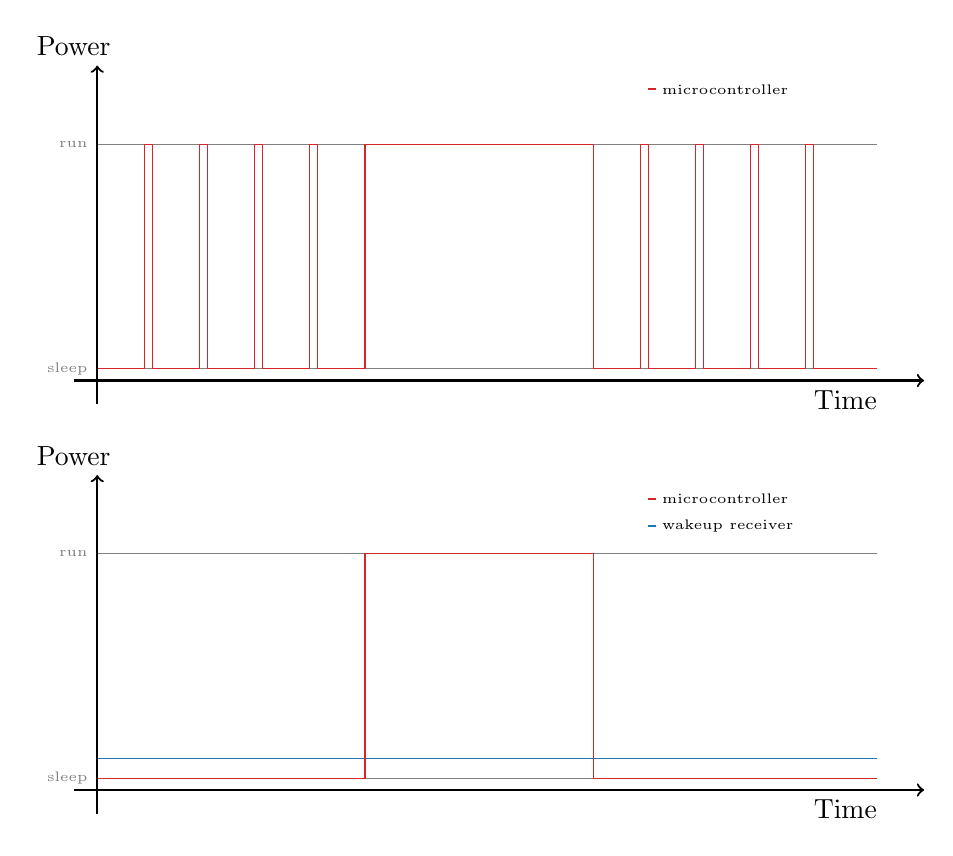
\begin{tikzpicture}
%oben
	%Modes
	\draw[gray] (0,0.15)--(9.9,0.15);
	\node[left, gray] at (0,0.15) {\tiny sleep};
	\draw[gray] (0,3)--(9.9,3);
	\node[left, gray] at (0,3) {\tiny run};
	
	
	%Plot
	\definecolor{pltred}{RGB}{214,39,40}
	
	\foreach \x in {0,0.7,1.4,2.1}
		\draw[pltred] (\x,0.15)--++(0.6,0)--++(0,2.85)--++(0.1,0)--++(0,-2.85);
	
	\draw[pltred] (2.8,0.15)--(3.4,0.15)--(3.4,3)--(6.3,3)--(6.3,0.15);
	
	\foreach \x in {6.3,7,7.7,8.4}
		\draw[pltred] (\x,0.15)--++(0.6,0)--++(0,2.85)--++(0.1,0)--++(0,-2.85);
		
	\draw[pltred] (9.1,0.15)--(9.9,0.15);
	
	%Koordinantenkreuz + Legende
	\draw[->, thick] (0,-0.3)--(0,4);
	\draw[->, thick] (-0.3,0)--(10.5,0);
	\node[above] at (-0.3,4) {Power};
	\node[below] at (9.5,0) {Time};
	\draw[thick, pltred] (7,3.7)--++(0.1,0);
	\node[right] at (7.05,3.7) {\tiny microcontroller};
	

%unten
	\def\sh{5.2}
	\definecolor{pltblue}{RGB}{31,119,180}
	%modes
	\draw[gray] (0,0.15-\sh)--(9.9,0.15-\sh);
	\node[left, gray] at (0,0.15-\sh) {\tiny sleep};
	\draw[gray] (0,3-\sh)--(9.9,3-\sh);
	\node[left, gray] at (0,3-\sh) {\tiny run};
	
	
	%Plot
	\draw[pltblue] (0,0.4-\sh)--(9.9,0.4-\sh);
	\draw[pltred] (0,0.15-\sh)--(3.4,0.15-\sh)--(3.4,3-\sh)--(6.3,3-\sh)--(6.3,0.15-\sh)--(9.9,0.15-\sh);
	
	%Koordinantenkreuz + Legende
	\draw[->, thick] (0,-0.3-\sh)--(0,4-\sh);
	\draw[->, thick] (-0.3,0-\sh)--(10.5,0-\sh);
	\node[above] at (-0.3,4-\sh) {Power};
	\node[below] at (9.5,0-\sh) {Time};
	\draw[thick, pltred] (7,3.7-\sh)--++(0.1,0);
	\node[right] at (7.05,3.7-\sh) {\tiny microcontroller};
	\draw[thick, pltblue] (7,3.35-\sh)--++(0.1,0);
	\node[right] at (7.05,3.35-\sh) {\tiny wakeup receiver};
	
	
	
\end{tikzpicture}		
\end{document}
